\documentclass[12pt,a4paper]{article}
\usepackage[utf8]{inputenc}
\usepackage[german]{babel}
\usepackage[T1]{fontenc}
\usepackage{amsmath}
\usepackage{amsfonts}
\usepackage{amssymb}
\usepackage{graphicx}
\usepackage{siunitx}
\usepackage{float}
\usepackage[left=2cm,right=2cm,top=2cm,bottom=2cm]{geometry}
\usepackage{hyperref}
\author{Gerald}

\begin{document}
\sisetup{separate-uncertainty = true}
	\setlength{\parindent}{0pt} 
	\begin{center}
		{\LARGE Versuchsprotokoll}\\
		\begin{large}
			zum Fortgeschrittenenpraktikum im Bachelorstudiengang Physik\\[0.4cm]
			an der RWTH Aachen\\
			II. Physikalisches Institut A\\[5.5cm]
			\Large\textbf{\textsl{Magnetische Phasenübergänge (PH)}}\\[5.5cm]
			\normalsize\textit{vorgelegt\\von}\\[0.4cm]
			\large{Moritz Berger (355244)\\Gerald Kolter (355005)}\\\textbf{Gruppe 30}\\[2cm]
			\large \textbf{Wintersemester 2017/18}
		\end{large}
	\end{center}
	\newpage
	
	\tableofcontents
	\newpage

\section{Versuchsziel}
Ziel des Versuchs ist es die Sprungtemperatur eines Hochtemperatursupraleiters und die Curie-Temperatur und dadurch die Zusammensetzung einer GdAg$_{1-x}$Zn$_x$-Probe zu bestimmen.

\section{Aufbau}
Der Messaufbau für den Hauptversuch besteht aus einem Hartshorn-Spulensystem, das zusammen mit der darin befindlichen Probe in flüssigem Stickstoff abgekühlt wird. Mit einem Lockin-Verstärker wird die Differenz zwischen den Signalen der beiden gegenläufigen Empfängerspulen gemessen und über ein Multimeter mit dem Messrechner angeschlossen. Unter dem Hartshorn-Spulensystem befindet sich eine Si-Diode zur Messung der Temperatur, die ebenfalls an den Messrechner angeschlossen ist.

\section{Durchführung}
\subsection{Vorversuche}
\subsubsection{Untersuchung eines Tiefpasses}

\begin{figure}
\centering
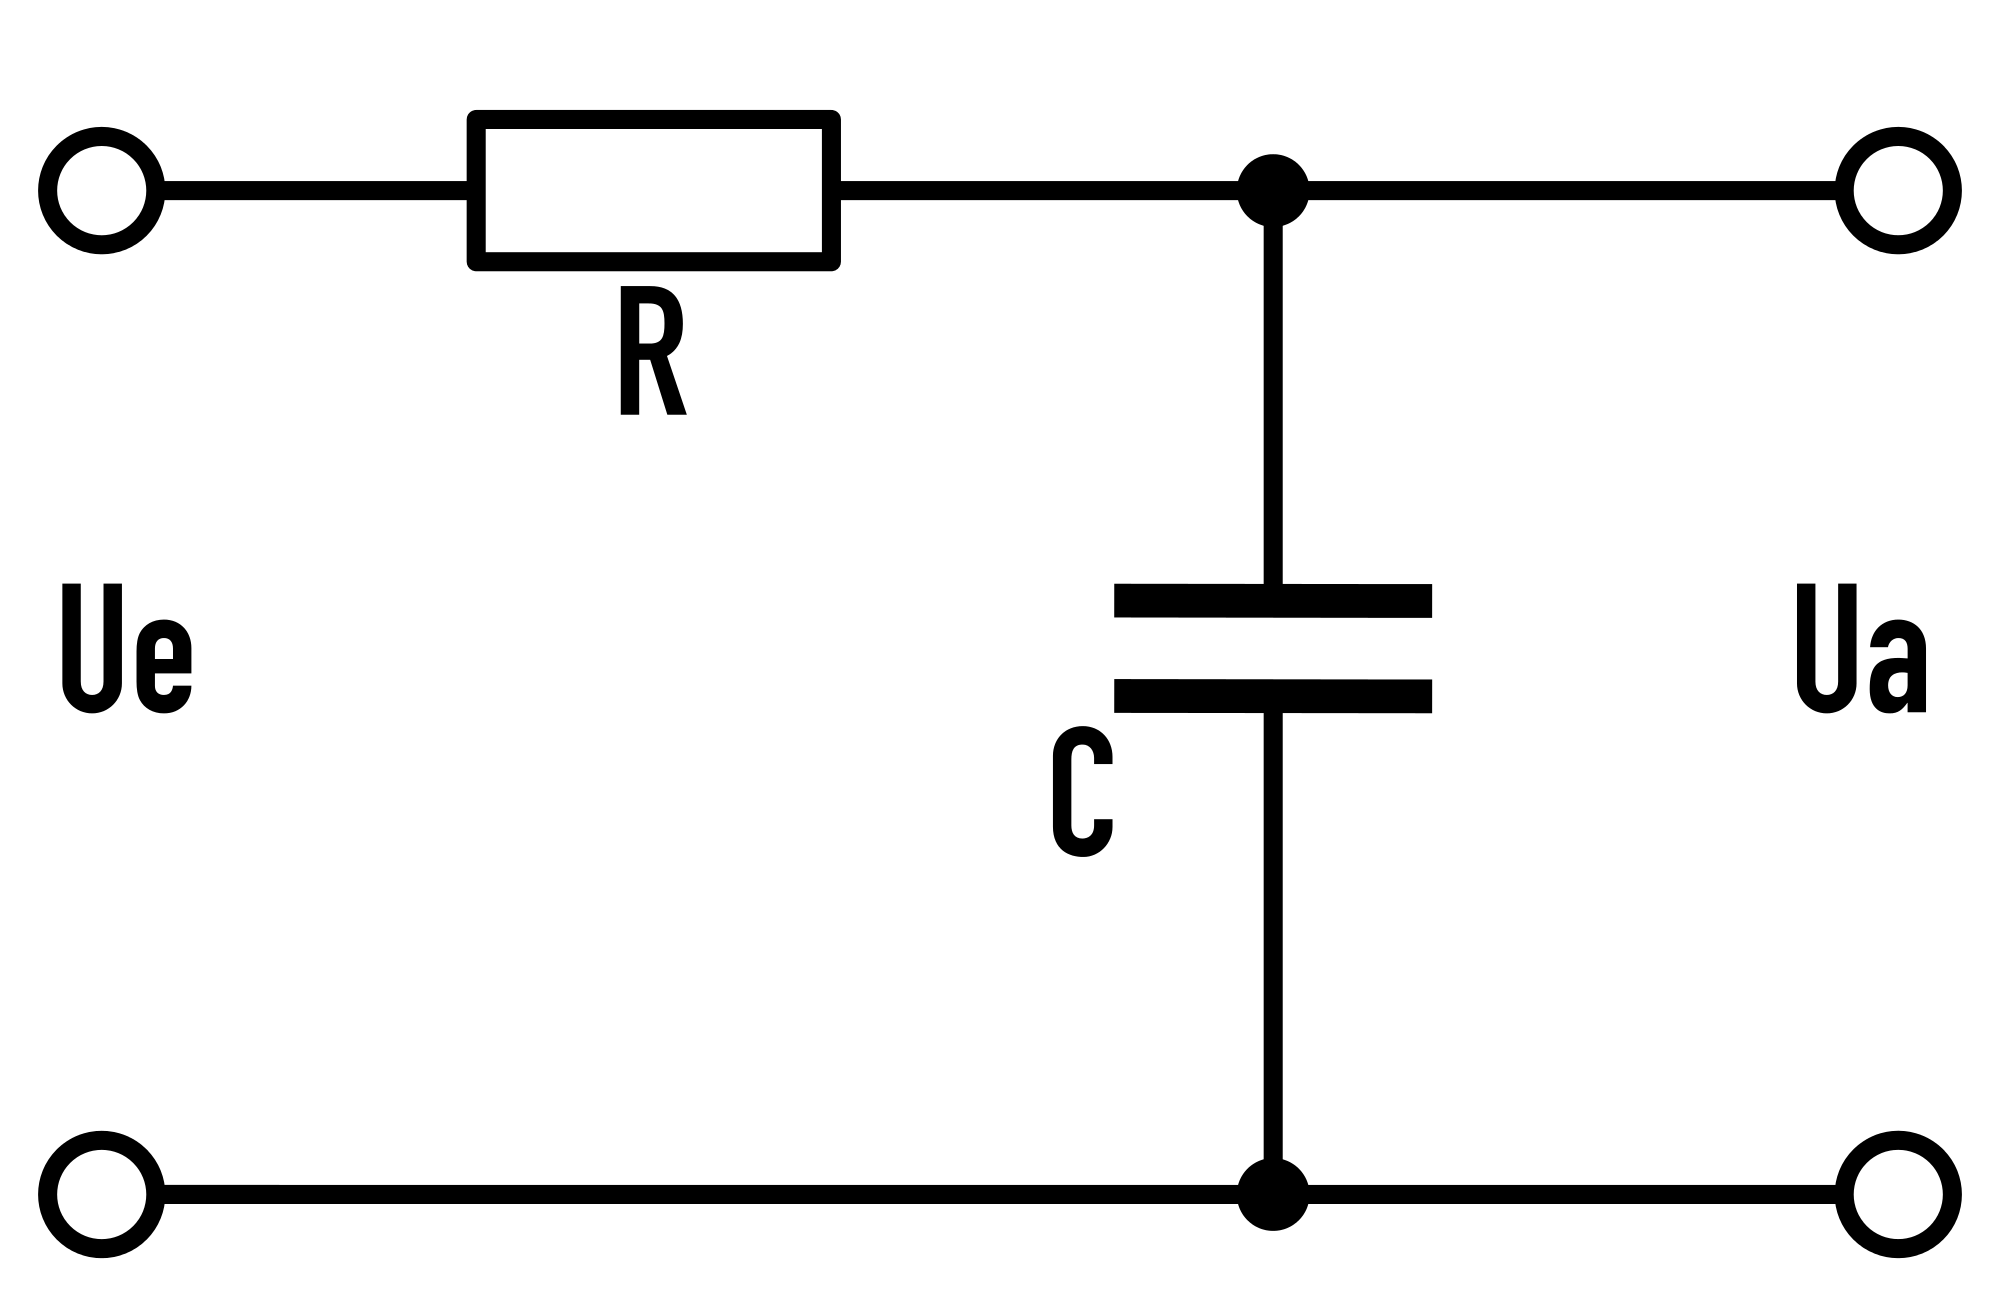
\includegraphics[scale=0.1]{Bilder/Vorversuch1/Tiefpass_Schaltbild.png}
\caption[test]{Schaltbild\footnotemark eines Tiefpasses.}
\label{fig:Tiefpass_Schaltbild}
\end{figure}
\footnotetext{Quelle: http://de.wikipedia.org/wiki/Tiefpass}

Mit einem $\SI{1,5}{k \Omega}$ Widerstand und einem $\SI{100}{nF}$ Kondensator wird ein Tiefpass zusammengesetzt. Mit einem Frequenzgenerator wird eine sinusförmige Wechselspannung an den Tiefpass angelegt. Abbildung \ref{fig:Tiefpass_Schaltbild} zeigt das entsprechende Schaltbild. Die angelegte Frequenz wird durchgefahren und dabei werden die an den Tiefpass angelegte und die durch den Tiefpass gefilterte Wechselspannung auf dem Oszilloskop gemessen.

\subsubsection{Untersuchung der Filter des Lockin-Verstärkers}
Das Referenzsignal des Lockin-Verstärkers wird auf einen Eingang des Lockin-Verstärkers gelegt. Die Filterfrequenz wird auf $f_0 = \SI{1000}{Hz}$ eingestellt. Es werden alle drei Filter (Tiefpass-, Hochpass- und Bandpassfilter) des Lockin-Verstärkers vermessen, indem jeweils die Frequenz des Referenzsignals durchgefahren und die Spannungsausgabe des Lockin-Verstärkers gemessen wird.

\subsubsection{Signalfiltern mit Tiefpass und Hochpass}
Mit einem Frequenzgenerator wird eine niedrige Frequenz erzeugt und an einen Eingang des Lockin-Verstärkers gelegt. An den anderen Eingang des Lockin-Verstärkers wird das Referenzsignal des Lockin-Verstärkers gelegt. Mit dem Oszilloskop werden sowohl das Signal des Frequenzgenerators, das Referenzsignal und die Überlagerung der beiden Signale, die der Lockin-Verstärker auf dem SIG.MON Ausgang ausgibt, betrachtet.\\

\subsubsection{Zeitkonstante und Empfindlichkeit}

\begin{table}
\centering
\begin{tabular}{|c|c|}
\hline 
Integrationszeit $T_I$ & \SI{10}{ms} \\ 
\hline 
Amplitude $U_0$ & \SI{0,5}{V} \\
\hline 
Verstärkung $s$ & \SI{200}{mV} \\ 
\hline 
Phasenschieber & $\varphi = \frac{\pi}{2}$ \\ 
\hline 
\end{tabular} 
\caption{Einstellungen zur Bestimmung einer geeigneten Zeitkonstanten und Empfindlichkeit.}
\label{tab:Zeitkonst_Einstellungen}
\end{table}

Der Lockin-Verstärker integriert das Signal über einen einstellbaren Zeitraum, um so die Schwingung aufgrund der Orthogonalitätsbedingung aus dem Ausgangssignal zu integrieren. \\
Die Empfindlichkeit $s$ des Lockin-Verstärkers wird angegeben in der Spannung, die auf \SI{10}{V} verstärkt wird, sodass sich der Verstärkungsfaktor zu $v = \frac{\SI{10}{V}}{s}$ berechnet. \\
Das Referenzsignal wird auf den Eingang des Lockin-Verstärkers gelegt. Die Frequenz des Referenzsignals wird durchgefahren, um ein geeignetes Verhältnis zwischen Referenzfrequenz und Integrationszeit zu finden. Tabelle \ref{tab:Zeitkonst_Einstellungen} zeigt die verwendeten Einstellungen.

\subsection{Hauptversuch}
\subsubsection{Messung des Supraleiters}

\begin{table}
\centering
\begin{tabular}{|c|c|}
\hline 
Integrationszeit $T_I$ & \SI{10}{ms} \\ 
\hline 
Sensitivität $s$ & \SI{500}{\mu V} \\ 
\hline
Filter & Bandpass \\
\hline
Güte & 1 \\
\hline
Filterfrequenz & \SI{380}{Hz} \\
\hline 
Phasenschieber & $\varphi$ = 84.5$^{\circ}$ \\ 
\hline 
\end{tabular} 
\caption{Einstellungen für die Messung des Supraleiters.}
\label{tab:Supra_Einstellungen}
\end{table}

Tabelle \ref{tab:Zeitkonst_Einstellungen} zeigt die Einstellungen, die für die Messungen mit dem Supraleiter verwendet wurden. \\
Der Messstab mit dem Supraleiter wird zunächst mit einer Pumpe evakuiert und anschließend mit Helium als Kontaktgas befüllt. Das Ende des Stabes, an dem die Messeinrichtung sitzt, wird zum Kühlen in einen mit flüssigem Stickstoff gefüllten Dewar getaucht und auf ca. \SI{80}{K} gekühlt. Für die Messung wird anschließend der Messstab aus dem Stickstoff herausgezogen, allerdings nur so weit, dass die Erwärmungsrate $\frac{\Delta T}{\Delta t}$ unter \SI{0,1}{K/s} bleibt. Dies ist wichtig, um sicherzustellen, dass zu jedem Zeitpunkt eine möglichst homogene Temperaturverteilung gegeben ist. Während der Erwärmung von \SI{80}{K} auf ca. \SI{120}{K} wird die Temperatur und die Differenzspannung zwischen den beiden Empfängerspulen des Hartshorn-Spulensystems gemessen. \\
Diese Messung wird einmal ohne Probe als Untergrundmessung zur Korrektur und zweimal mit dem Supraleiter durchgeführt: Einmal mit einer Phasenverschiebung zwischen Eingangssignal und Referenzsignal des Lockin-Verstärkers von $\varphi = 0$ und einmal mit einer Phasenverschiebung von $\varphi = \frac{\pi}{2}$, sodass der Realteil ($\varphi = 0$) und der Imaginärteil ($\varphi = \frac{\pi}{2}$) der Suszeptibilität gemessen werden.

\subsubsection{Messung der Probe}
Bei der Vermessung der GdAg$_{1-x}$Zn$_x$-Probe wird nur der Imaginärteil gemessen. Die Messung wurde ebenfalls bei ca. \SI{80}{K} gestartet, jedoch bis ca. \SI{190}{K} aufgenommen. Aufgrund eines betragsgroßen Offset war der Betrag der an den Lockin-Verstärker angelegten Spannung zu groß, sodass hier die Sensitivität auf \SI{1}{mV} erhöht werden musste.

\section{Ergebnisse}
\subsection{Vorversuche}
\subsubsection{Untersuchung eines Tiefpasses}
\subsubsection{Untersuchung der Filter des Lockin-Verstärkers}


\subsubsection{Signalfiltern mit Tiefpass und Hochpass}
\begin{figure}
\centering
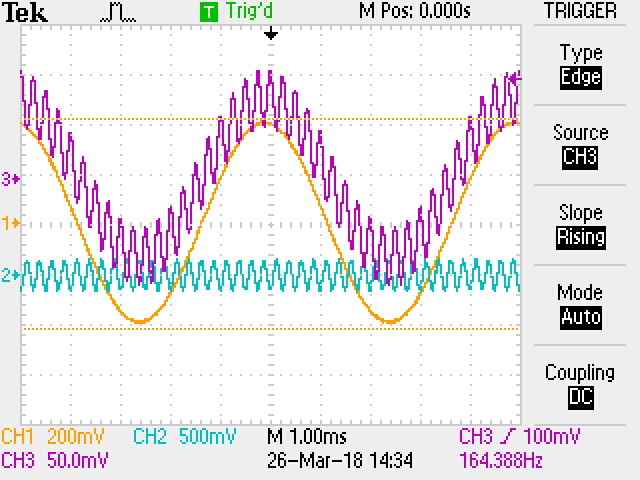
\includegraphics[scale=0.9]{Bilder/Vorversuch3/F0000TEK.JPG}
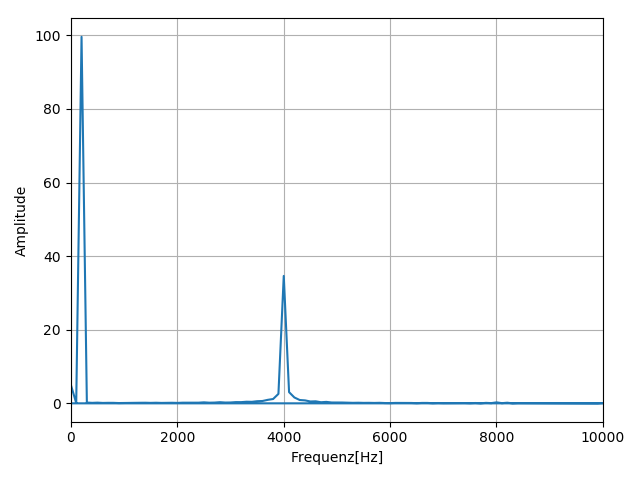
\includegraphics[scale=0.5]{Bilder/Vorversuch3/Vor3_0.png}
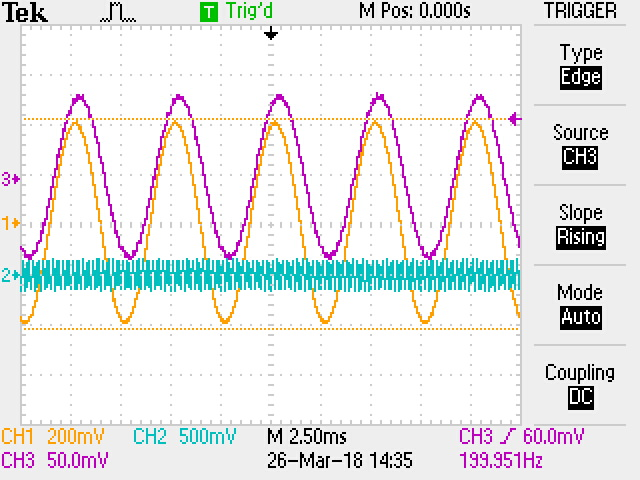
\includegraphics[scale=0.9]{Bilder/Vorversuch3/F0001TEK.JPG}
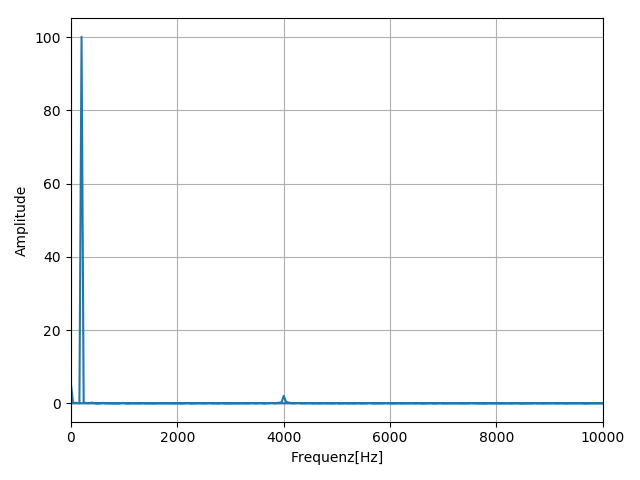
\includegraphics[scale=0.5]{Bilder/Vorversuch3/Vor3_1.png}
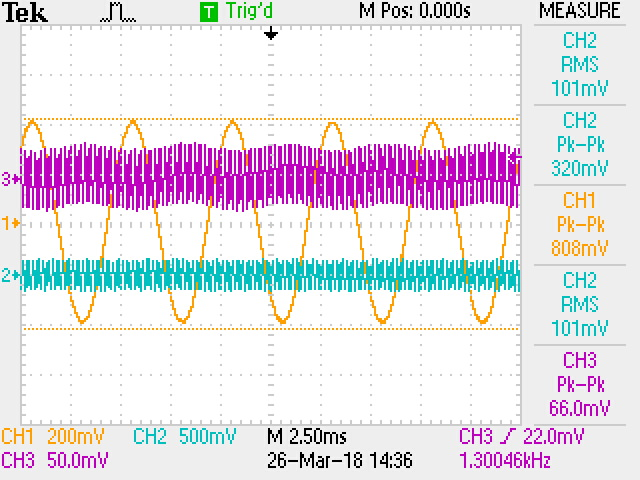
\includegraphics[scale=0.9]{Bilder/Vorversuch3/F0002TEK.JPG}
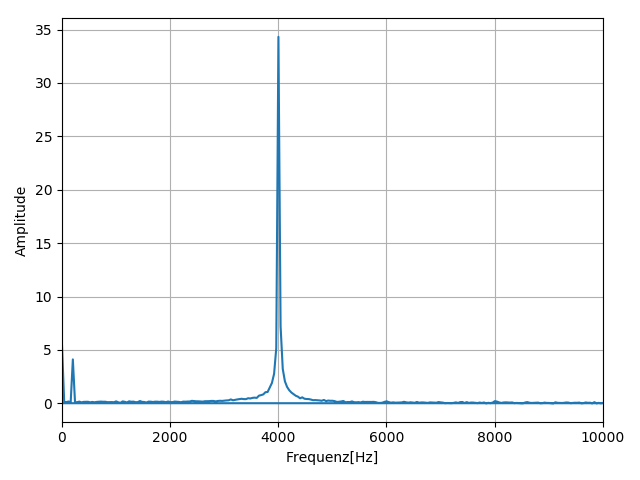
\includegraphics[scale=0.5]{Bilder/Vorversuch3/Vor3_2.png}
\caption{Osziloskopbilder zum Vorversuch zum Signalfiltern (Filterfrequenz: 1000Hz). \textbf{Oben:} Flat (kein Filter), \textbf{mitte:} Tiefpass, \textbf{unten:} Hochpass.
In allen Bildern ist an CH1 (orange) die kleine Frequenz (200Hz), CH2 (blau) die große Frequenz (4000Hz) und an CH3 die gefilterte Überlagerung der beiden Frequenzen angelegt.}
\label{fig:Vor3_Oszi}
\end{figure}

\begin{figure}
\centering
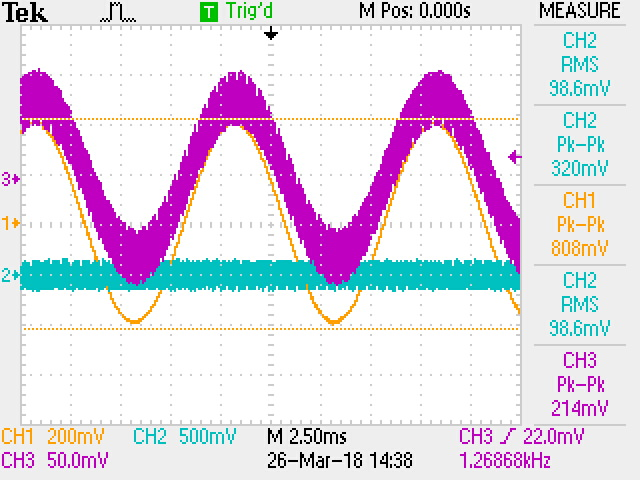
\includegraphics[scale=0.9]{Bilder/Vorversuch3/F0003TEK.JPG}
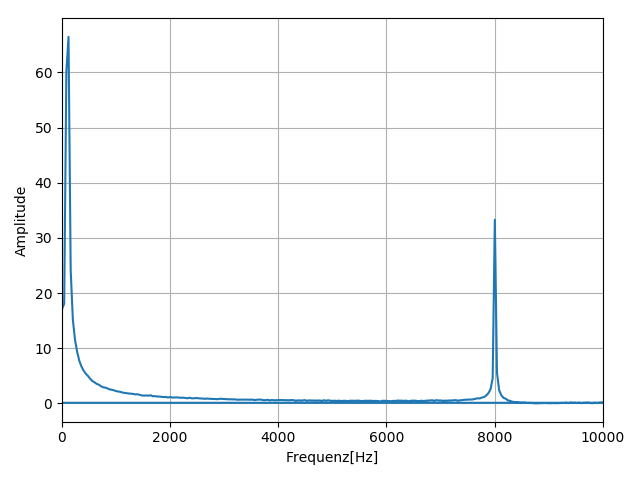
\includegraphics[scale=0.5]{Bilder/Vorversuch3/Vor3_3.png}
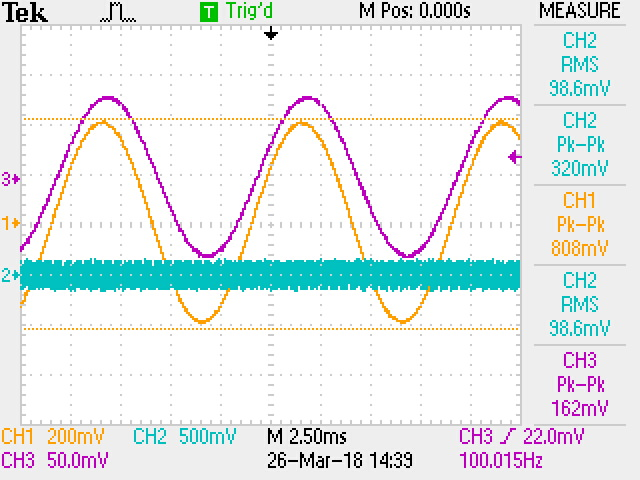
\includegraphics[scale=0.9]{Bilder/Vorversuch3/F0004TEK.JPG}
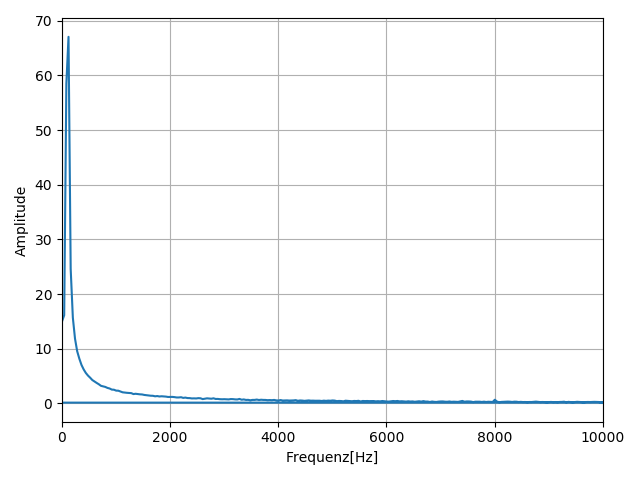
\includegraphics[scale=0.5]{Bilder/Vorversuch3/Vor3_4.png}
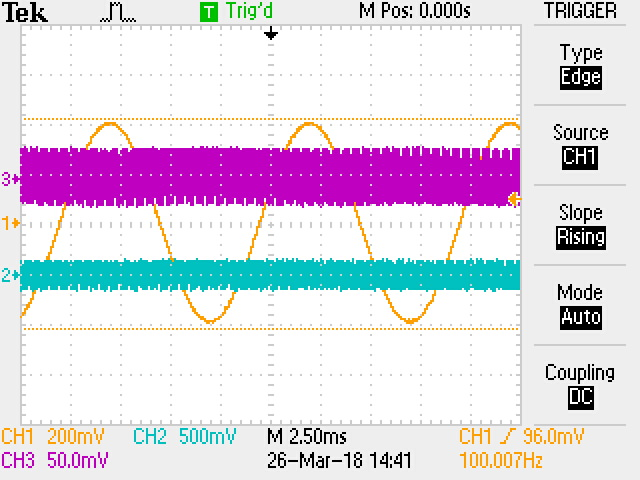
\includegraphics[scale=0.9]{Bilder/Vorversuch3/F0005TEK.JPG}
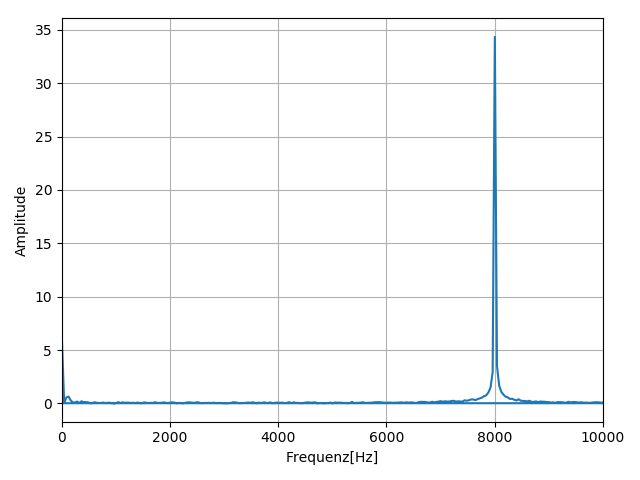
\includegraphics[scale=0.5]{Bilder/Vorversuch3/Vor3_5.png}
\caption{Osziloskopbilder zum Vorversuch zum Signalfiltern(Filterfrequenz: 1000Hz). \textbf{Oben:} Flat (kein Filter), \textbf{mitte:} Tiefpass, \textbf{unten:} Hochpass.
In allen Bildern ist an CH1 (orange) die kleine Frequenz (100Hz), CH2 (blau) die große Frequenz (8000Hz) und an CH3 die gefilterte Überlagerung der beiden Frequenzen angelegt.}
\label{fig:Vor3_Oszi2}
\end{figure}

\begin{table}
\centering
\begin{tabular}{|c|c|c|c|}
\hline
Filter & Frequenz & Höhe & rel. Höhe\\
\hline
kein & 100 & 66.4 & 1\\
\cline{2-4}
& 200 & 99.6 & 1\\
\cline{2-4}
& 4000 & 34.6 & 1\\
\cline{2-4}
& 8000 & 33.3 & 1\\
\hline
\hline
Tiefpass & 100 & 67.1 & 1.01\\
\cline{2-4}
& 200 & 100.1 & 1.01\\
\cline{2-4}
& 4000 & 2.1 & 0.06\\
\cline{2-4}
& 8000 & 0.7 & 0.02\\
\hline
\hline
Hochpass & 100 & 5.7 & 0.08\\
\cline{2-4}
& 200 & 4.1 & 0.04\\
\cline{2-4}
& 4000 & 34.3 & 0.99\\
\cline{2-4}
& 8000 & 34.3 & 1.03\\
\hline
\end{tabular} 
\caption{Ergebnisse der Peakhöhen der FFT-Spektren. Angegeben ist jeweils der verwendete Filter, die Frequenz, die absolute Peakhöhe (der genaue Wert hat keine Aussage) und die relative Peakhöhe verglichen mit den Höhen ohne Filter.}
\label{tab:Peakhohen}
\end{table}

In Abbildung \ref{fig:Vor3_Oszi} sind die Oszilloskopbilder für die Frequenzen 200Hz und 4000Hz zu sehen und in Abbildung \ref{fig:Vor3_Oszi2} die für die Frequenzen 100Hz und 8000Hz. Zur besseren Auswertung wurde jeweils eine Fast Fourier Transformation der dazugehörigen Daten durchgeführt. Diese ist jeweils neben dem Oszilloskopbild zu sehen. Aus den FFT-Spektren wurde die Peakhöhe abgelesen. Die Werte sind in Tabelle \ref{tab:Peakhohen} aufgelistet.\\
\\
Bei den Aufnahmen ohne Filter (jeweils das oberste Bild) sieht man wie erwartet eine Überlagerung beider Frequenzen. Dabei ist die Intensität der niedrigen Frequenz deutlich höher. Dies liegt aber einfach daran, dass das Eingangsignal auf eine größere Amplitude eigestellt war.\\
\\
Bei den Aufnahmen mit dem Tiefpass ist die hohe Frequenz deutlich abgeschwächt und wird nurnoch mit einer relativen Höhe im einstelligen Prozentbereich registriert. Sie fällt zwischen der 4000Hz und 8000Hz Messung sogar nochmal um einen Faktor 3. Diese Abschwächung stimmt mit dem erwarteten Modell aus dem vorherigen Vorversuch überein. Die kleine Frequenz wird hier sogar ganz leicht verstärkt [GÜTE???]...\\
\\
Beim Hochpass ist dies wie erwartet genau anders herum. Hier werden die kleinen Frequenzen abgeschwächt. Die relative Höhe ist hier etwas ungenauer, da nur wenige Perioden in den Daten vorhanden sind. Deswegen ist hier auch der 100Hz Peak etwas stärker ausgeprägt als der 200Hz Peak.\\
Im Bild mit der 200Hz Frequenz (Abbildung \ref{fig:Vor3_Oszi} unteres Bild) kann man ausßerdem sehen, dass die kleine Frequenz um c.a $180^\circ$ phasenverschoben gegenüber der Eingangsfrequenz ist. Dies stimmt auch mit den Ergebnissen aus dem vorherigen Vorversuch überein. Leider ist die Auflösung der hohen Frequenz zu gering, sonst würde man dises Phänomen vermutlich auch beim Tiefpass bei der hohen Frequenz feststellen. 


\subsubsection{Zeitkonstante und Empfindlichkeit}
Aus den Messeinstellungen ergibt sich ein in diesem Versuch verwendeter Verstärkungsfaktor von $v = 50$. Man erhält also die eigentlich gemessene Spannung, indem man die abgelesene verstärkte Spannung durch 50 teilt. In Abbildung \ref{fig:Vor4} sind die aufgenommenen Datenpunkte gegen die Frequenz aufgetragen. Die Spannungen haben immer um c.a 0.1V geschwankt, weswegen ein Ablesefehler von $0.1/50/\sqrt{12}$ auf die echten Spannungswerte angenommen wurde.\\
Zur besseren Auswertung wurde eine Anpassung an die Daten durchgeführt. Diese ist in Abbildung \ref{fig:Vor4_anpassung} zu sehen. Dabei stellt sich heraus, dass die Daten sehr gut einer $1/x^2$-Funktion folgen.\\
\\
Nun möchte man das optimale Verhältnis zwischen Integrationszeit $T_I$ und der Peraiodendauer T wissen, wobei gilt:
\begin{equation}
Ver = \dfrac{T_I}{T} = T_I \cdot f
\end{equation}
Während des Versuches wurde abgeschätzt, dass für die verwendete Integrationszeitvon $T_I = \SI{10}{ms}$ mindestens eine Frequenz von $f = \SI{1500}{Hz}$ benutzt werden muss, da sich die Werte ab dieser Frequenz kaum noch ändern. Dies führt zu einem schnell abgeschätzen Verhältnis von $Ver = 15$.\\
Beim Hauptversuch entstehen Spannungen im $\si{\mu V}$ Bereich (Empfindlichkeit auf $s = 500\mu V$ eingestellt). Der Einfluss auf die maximale Spannung durch die Integrationszeit sollte unter $1\%$ betragen, also einem Spannungsoffset von $5\mu V$. Es wird also visuell abgeschätzt, wann die Anpassung unter diesen Offset läuft(nach Abzug des Offsets (Anpassungsparameter d) der Anpassung, also wird nach einem y-Wert von $(0.0122\pm 0.0002)mV$ gesucht).  Dies ist der Fall bei $f = \SI{1610\pm 20}{Hz}$ (mit Ablesefehler). Daraus ergibt sich ein \textbf{minimales} Verhältnis von
\begin{equation*}
\boxed{T_I \cdot f = 16.1\pm 0.2}
\end{equation*}
Im Hauptversuch wurde eine Frequenz von \SI{380}{Hz} verwendet. Man benötigt also eine Integrationszeit von \SI{100}{ms}, da das Verhältnis sonst zu klein ist. Mit diesen Einstellungen ergibt sich ein Verhältnis von 
$38$. Die Bedingung ist also sehr gut erfüllt.
\begin{figure}
\centering
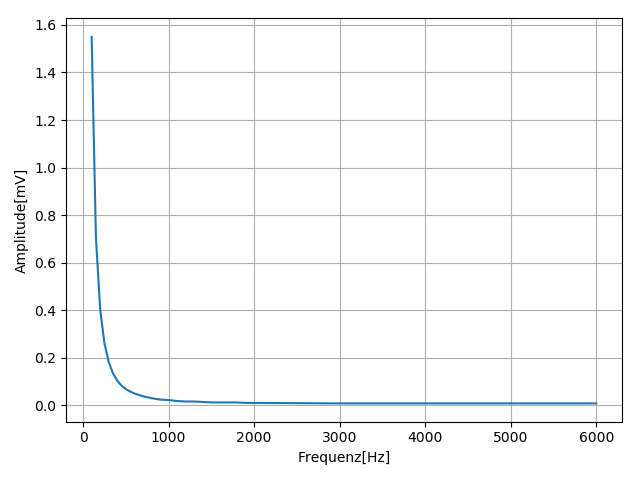
\includegraphics[scale=0.8]{Bilder/Vorversuch4/Vor4_0.png}
\caption{Aufgenommene Datenpunkte zur Betrachtung der Integrationszeit (T=10ms). Es wurde das echte Eingangsignal($U_{gemessen}/50$) gegen die Frequenz aufgetragen.}
\label{fig:Vor4}
\end{figure}

\begin{figure}
\centering
\includegraphics[scale=0.8]{Bilder/Vorversuch4/Vor4_1.png}
\includegraphics[scale=0.8]{Bilder/Vorversuch4/Vor4_2.png}
\caption{Anpassung an die Daten zur Zeitkonstante und eine Vergrößerung in den relevanten Bereich.}
\label{fig:Vor4_anpassung}
\end{figure}

\subsection{Hauptversuch}
\subsection{Messung des Supraleiters}
\subsubsection{Phasenkalibration}
\begin{figure}
\centering
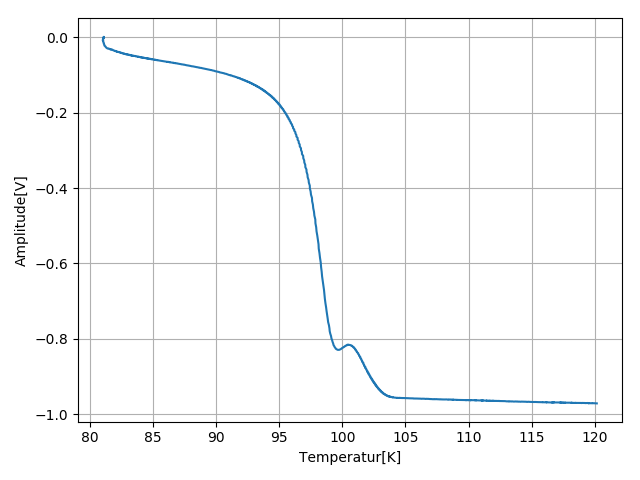
\includegraphics[scale=0.5]{Bilder/Haupt_Supra/Kalialt.png}
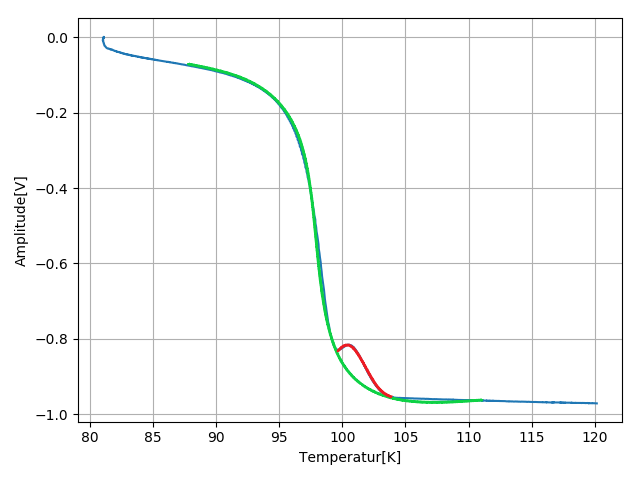
\includegraphics[scale=0.5]{Bilder/Haupt_Supra/Kalialt_2.png}
\caption{Ursprüngliche Phasenkalibration, bei der die Spannung mithilfe der Phase auf 0 kalibriert wurde. Im rechten Bild wurde der Verlauf von $\chi'$ in grün und der von $\chi''$ in rot gekennzeichnet.}
\label{fig:Supra_Kalialt}
\end{figure}


Um Real- und Imaginärteil möglichst unabhängig voneinander betrachten zu können muss die Phase möglichst genau auf $90^\circ$ bzw. auf $0^\circ$ kalibriert werden. Ursprünglich sollte dies mithilfe der Tatsache geschehen, dass für den Supraleiter
\begin{equation}
\chi_C = -1-i\cdot 0
\end{equation}
gilt, der Imaginärteil also 0 ist.\\
Man verucht also auf $90^\circ$ so zu kalibrieren, dass der Offset \SI{0}{V} beträgt. Eine Messreihe mit einer solchen Kalibration ist in Abbildung \ref{fig:Supra_Kalialt} dargestellt.\\
Das Problem dabei ist, dass die Position des Dewar-Gefäßes das Magnetfeld der Spulen beeinflusst. Da diese Postition mehrfach während des Versuches geändert werden muss, entsteht ein Offset, der nicht durch das Potentiometer ausgeglichen wurde. Den Einfluss kann man zum Beispiel durch eine Änderung in der Spannung ganz am Anfang der Messung beobachten, wo das Spulensystem leicht aus dem Dewar angehoben wird, um den Erwärmungsvorgang zu starten.\\
Bei der 0-Kalibration kalibriert man somit nicht auf $90^\circ$, sondern auf irgendeinen anderen Wert. Dies zeigt sich in Abbildung \ref{fig:Supra_Kalialt} durch das gleichzeitige Auftreten der $\chi'$-Kurve (Änderung von $\chi' = -1$ zu $\chi' << 1$ an der kritischen Temperatur) und des $\chi''$-Peaks.\\
\\
Um die Phase besser kalibriern zu können wurde ein alternatives Vervahren verwendet. Es wurde zuerst für eine Phase von $90^\circ$ ein Kurvenverlauf aufgezeichnet und dann geschaut, wie sich dieser Verlauf ändert, wenn man die Phase leicht verringert. Dies wird solange wiederholt, bis der Unterschied vor und hinter der Sprungtemperatur, der durch die $\chi'$-Kurve entsteht, verschwindet. Dieses Verfahren ist in Abbildung \ref{fig:Supra_Kali} anhand von 4 Schritten dargestellt.

\begin{figure}
\centering
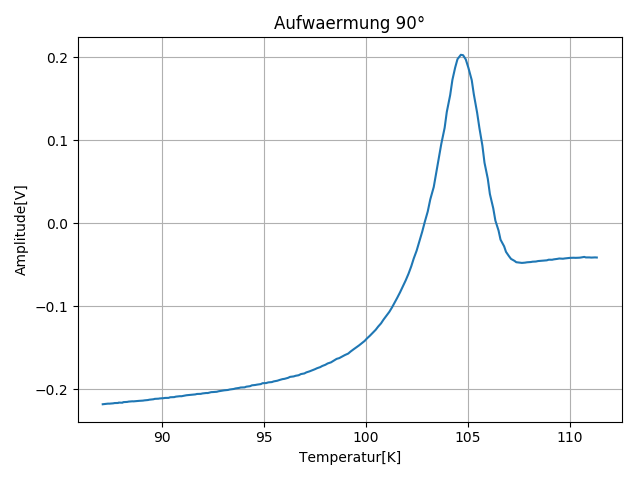
\includegraphics[scale=0.5]{Bilder/Haupt_Supra/Kal_2.png}
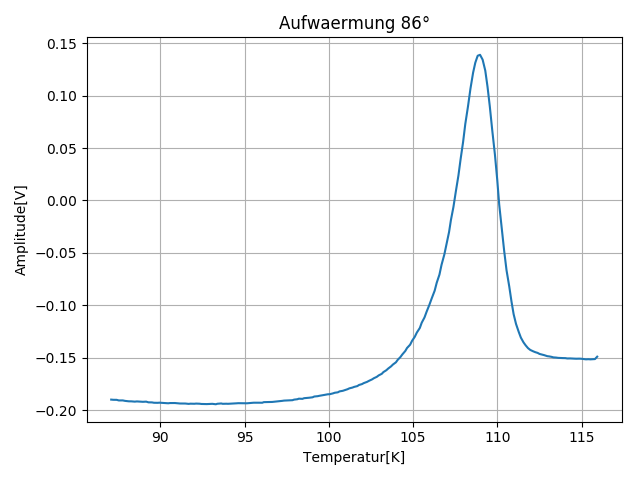
\includegraphics[scale=0.5]{Bilder/Haupt_Supra/Kal_0.png}
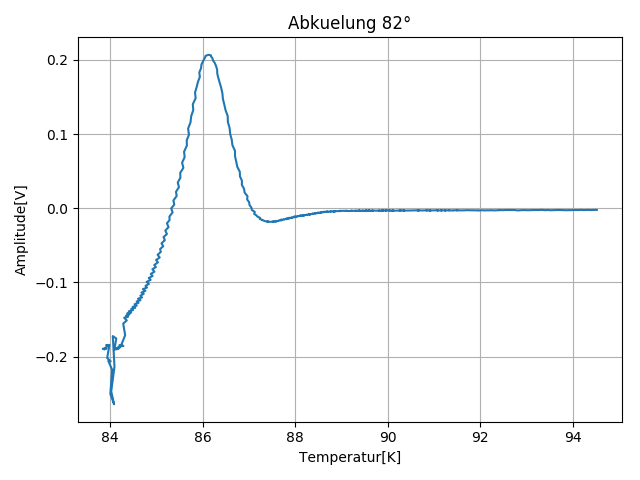
\includegraphics[scale=0.5]{Bilder/Haupt_Supra/Kal_1.png}
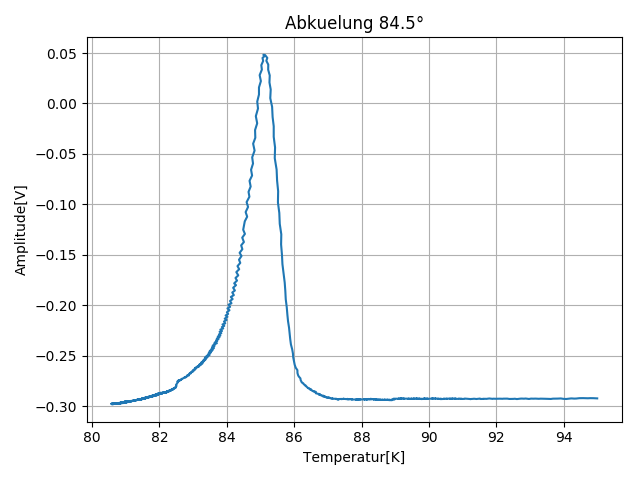
\includegraphics[scale=0.5]{Bilder/Haupt_Supra/Kal_3.png}
\caption{Alternative Phasenkalibration. \textbf{Oben links:} Aufwärmvorgang mit Phaseneinstellung von $90^\circ$. Der Verlauf der $\chi'$-Kurve ist sichtbar. \textbf{Oben rechts:} Aufwärmvorgang mit etwas besserer Phase von $86^\circ$. $\chi'$-Kurve ist schwächer ausgeprägt. \textbf{Unten links:} Abkühlvorgang mit zu kleiner Phase von $82^\circ$. $\chi'$-Kurve ist wieder stärker ausgeprägt. \textbf{Unten rechts:} Abkühlvorgang mit entgültiger  Phase von $82^\circ$. Die Spannung hat vor und hinter dem Peak den gleichen Wert.}
\label{fig:Supra_Kali}
\end{figure}

\subsubsection{Untergrundmessung}
\begin{figure}
\centering
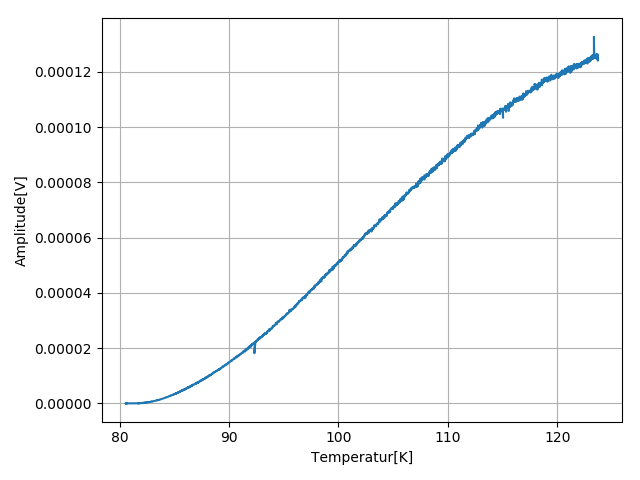
\includegraphics[scale=0.8]{Bilder/Haupt_Supra/Untergrund.png}
\caption{Untergrundmessung mit leerem Probenbehälter.}
\label{fig:Supra_Untergrund}
\end{figure}

In Abbildung \ref{fig:Supra_Untergrund} ist die Untergundmessung dargestellt. Am Anfang der Messung (bei nirdrigen Temperaturen) sieht man einen plötzlichen Anstieg der gemessenen Spannung. Dieser entsteht weider dadurch, dass der Stab leicht aus dem Dewar-Gefäß angehoben wird. Aus diesem Grund können nur Messwerte ab c.a 81.5K benutzt werden, falls ein Untergrundabzug durchgeführt wird.\\
Oberhalb dieser Temperatur folgen die Daten keinem einfachen Modell. Da die genaue Ursache dieses Verhaltens unbekannt ist, konnte keine Anpassung an die Daten durchgeführt werden. Stattdessen wird der Untergrund direkt von den Messreihen abgezogen.

\subsubsection{Auswertung der $\chi'$-Messung}
\begin{figure}
\centering
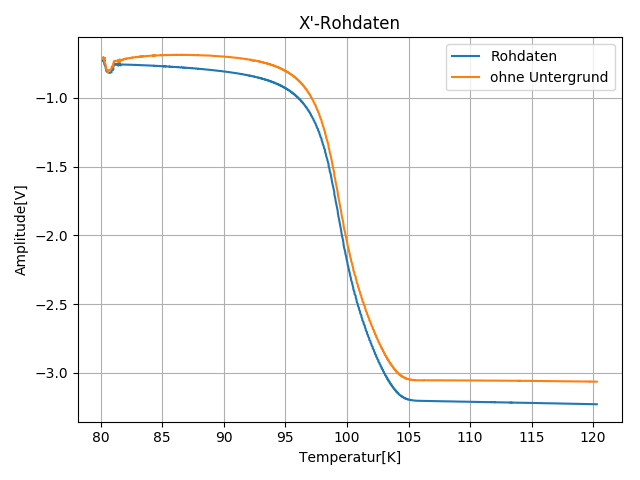
\includegraphics[scale=0.8]{Bilder/Haupt_Supra/X1roh.png}
\caption{Rohdaten der $\chi'$-Messung}
\label{fig:Supra_X1roh}
\end{figure}

\begin{figure}
\centering
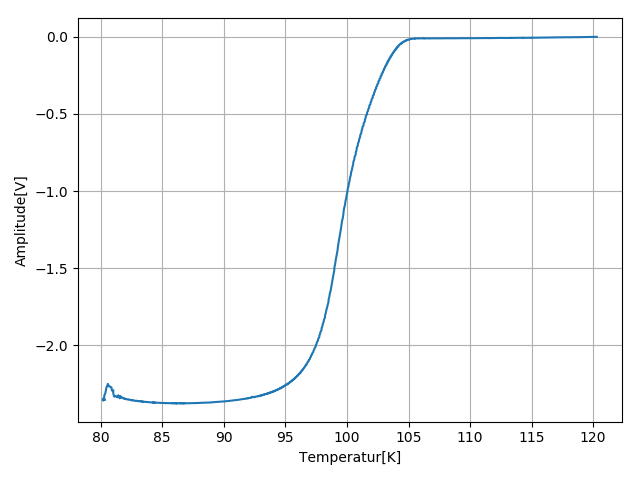
\includegraphics[scale=0.8]{Bilder/Haupt_Supra/X1_spiegel.png}
\caption{Vom Untergund korrigierte, gespiegelte und vom Offset bereinigte Daten der $\chi'$-Messung. Die y-Achse ist hier ansatzweise proportional zur Suszebtiblität.}
\label{fig:Supra_X1spiegel}
\end{figure}

\begin{figure}
\centering
\includegraphics[scale=0.5]{Bilder/Haupt_Supra/X1unten.png}
\includegraphics[scale=0.5]{Bilder/Haupt_Supra/X1oben.png}
\caption{Struktur in den "Plateaus" vor (linkes Bild) und hinter (rechtes Bild) in den Daten. Der Anpassungsbereich ist mit senkrechten Linien gekennzeichnet und liegt für den vorderen Berecih zwischen 82-87K und für den hinteren Bereich zwischen 107-120K.}
\label{fig:Supra_X1struct}
\end{figure}

Die Rohdaten der $\chi'$-Messung und die vom Untergrund bereinigten Daten sind in Abbildung \ref{fig:Supra_X1roh} dargestellt.\\
Da für diese Messung statt einer Phase von $0^\circ$ eine von $180^\circ$ verwendet wurde, sind die Daten an der X-Achse gespiegelt. Außerdem entsteht in dieser Messung ein relativ großer Offset.\\
Für $T>T_C$ ist der Supraleiter dia- oder paramagnetisch, es gilt also $|\chi'| << 1$. Falls man annimmt, dass für diese Temperaturen $|\chi'| \approx 0$ gilt, so kann man den Offset korrigieren. Da diese Korrektur für die Auswertung nicht relevant ist, wird sie nur durch abschätzen durchgeführt.
Die vom Untergund korrigierten, gespiegelten und vom Offset bereinigten Daten sind in Abbildung \ref{fig:Supra_X1spiegel} dargestellt. 

\paragraph{Bestimmung der Kalibrationskonstante}
Mit dem Wissen, dass $|\chi'| << 1$ für $T>T_C$ und $\chi' = 1$ für $T<T_C$ gilt, kann man die Kalibrationskonstante bestimmen. Dazu wird die Differenz der Spannungen vor und hinter dem Phasenwechsel gebildet.\\
Nach Abzug der Untergrundmessung bilden sich aber vor und hinter dem Phasenwechsel keine Plateaus aus. Stattdessen existiert immernoch eine Struktur in den Daten (vgl. Abbildung \ref{fig:Supra_X1struct}), welche die Bestimmung der jeweiligen Spannungen schwierig macht. Diese Sturktur kommt hauptsächlich dadurch, dass sich der Untergrund durch das Einbringen des Supraleiters leicht geändert hat.\\
Um trotzdem die Spannungsdifferenz ausrechnen zu können wird der Mittelwert dieser Plateaus gabildet. Die dafür ausgewählten Bereiche und die Position des Mittelwertes sind ebenfalls in Abbildung \ref{fig:Supra_X1struct} abgebildet.\\
\\
Der Bereich unter der Sprungtemperatur wurde so gewählt, dass die Streuung am Anfang vollständig rausgeschnitten wird und der Anstieg durch die Sprungstelle möglichst keinen Einfluss hat. Diese Systematik beginnt ungefähr an der Stelle, an der die Spannung wieder anfängt zu steigen, anstatt abzufallen. Für den Bereich oberhalb der Sprungstelle wurde möglichst das ganze Plateau betrachtet, wobei eine kleine Bufferzone ausgelaasen wurde, um sicherzustellen, dass das Plateau wirklich erreicht wurde.\\
\\
Wegen der Struktur sind die Werte aber nicht gaußisch verteilt, und man kann den Fehler der Werte nicht durch Standardabweichung erhalten. Stattdessen wird eine Gleichverteilung zwischen dem Maximum und Minimum des ausgewählten Bereiches angenommen, da keine Aussage darüber getroffen werden kann, in welche Richtung die Daten durch den Untergrund verschoben werden. Die Spannungswerte sind in Tabelle \ref{tab:X1_const} aufgelistet.\\
Es gilt:
\begin{equation}
\Delta U = C \cdot v \cdot V_{Supra} \cdot \Delta\chi
\end{equation}
mit der Spannungsdifferenz U, der Kalibrationskonstante C, dem Verstärkungsfaktor $v=20000$ und des Volumens des Supraleiters $V_{Supra} =\SI{ 14.7\pm 0.3}{mm^3}$. Auf das Volumen wurde ein Gleichverteilungsfehler von $0.1/\sqrt{12}mm^3$ angenommen. Unter der Annnahme, dass $\Delta\chi \approx 1$ gilt, kann man daraus die Kalibrationskonstante berechnen:
\begin{equation}
C = \dfrac{\Delta U}{v\cdot V_{Supra}}
\end{equation}
Alle Fehler werden dabei gaußisch fortgepflanzt. Daraus erhält man das Endergebnis von
\begin{equation*}
C = \SI{8034.2\pm 34.7}{Vm^{-3}}
\end{equation*}

\begin{table}
\centering
\begin{tabular}{|c|c|}
\hline 
Messgröße & Wert \\ 
\hline 
Spannung unteres Plateau & \SI{-2.368\pm 0.009}{V} \\ 
\hline 
Spannung oberes Plateau & \SI{-0.006\pm 0.003}{V} \\ 
\hline 
Spannungsdifferenz & \SI{2.362\pm 0.009}{V} \\ 
\hline 
Kalibrationskonstante & \SI{8034.2\pm 34.7}{Vm^{-3}} \\ 
\hline 
\end{tabular} 
\caption{•}
\label{tab:X1_const}
\end{table}

\paragraph{Bestimmung der Sprungtemperatur}
Die Spungtemperatur befindet sich gerade an der Stelle, an der die Suszeptiblität am stäksten zunimmt. Deswegen wird jedem Messpunkt eine Steigung zugewiesen, indem eine lineare Anpassung an einen bestimmten Bereich um den Messpunkt herum angepasst wird. So kann man den Messpunkt bestimmen, an dem der Datenverlauf am steilsten ansteigt. In Tabelle \ref{tab:X1_anpassungen} sind die Ergebnisse der Anpassungen rund um die steilste Stelle aufgelistet. In Abbildung
\ref{fig:Supra_X1anpass} sind die Anpassungen zur steilsten Stelle und jeweils 2 Nachbarpunkten visualisiert.\\
Für den Anpassungsbereich wurden jeweils die nächsten 10 Nachbarpunkte in beide Richtungen gewählt, da sich die Stelle maximaler Steigung ab dieser Anpassungsgröße nicht mehr verändert. In Abbildung \ref{fig:Supra_X1anpassgross} ist die Auswrikung eines größeren Anpassungsbereiches mit 20 Nachbarpunkten gezeigt.\\
\\
Innerhalb der Fehler der Anpassungen liegen die beiden nächsten Nachabrpunkte im Berecih der maximalen Spannung. Deswegen wurden sie bei der Fehlerabschätzung berücksichtigt, indem gesagt wird, dass diese Werte den Fahler bestimmen. Dadurch ergibt sich ein Endergebnis von
\begin{equation*}
T_C = (99.38^{+0.04}_{-0.06}) K
\end{equation*}

\begin{table}
\centering
\begin{tabular}{|c|c|c|c|c|}
\hline
& $ 99.24 \pm 0.01 $ & $ 0.486 \pm 0.004 $ & $ -49.646 \pm 0.365 $ & $ 9.6 $\\
\hline
& $ 99.27 \pm 0.01 $ & $ 0.486 \pm 0.004 $ & $ -49.629 \pm 0.366 $ & $ 9.67 $\\
\hline
& $ 99.32 \pm 0.01 $ & $ 0.491 \pm 0.004 $ & $ -50.055 \pm 0.357 $ & $ 8.93 $\\
\hline
\hline
& $ 99.38 \pm 0.01 $ & $ 0.493 \pm 0.004 $ & $ -50.264 \pm 0.366 $ & $ 9.2 $\\
\hline
\hline
& $ 99.42 \pm 0.01 $ & $ 0.489 \pm 0.004 $ & $ -49.954 \pm 0.4 $ & $ 11.19 $\\
\hline
& $ 99.47 \pm 0.01 $ & $ 0.486 \pm 0.004 $ & $ -49.632 \pm 0.368 $ & $ 9.6 $\\
\hline
& $ 99.51 \pm 0.01 $ & $ 0.485 \pm 0.004 $ & $ -49.526 \pm 0.398 $ & $ 11.21 $\\
\hline
\end{tabular} 
\caption{Ergebnisse }
\label{tab:X1_anpassungen}
\end{table}

\begin{figure}
\centering
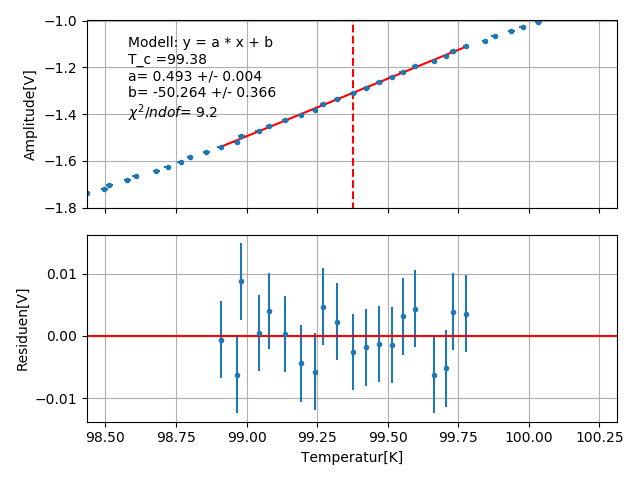
\includegraphics[scale=0.8]{Bilder/Haupt_Supra/X1_Steigung.png}
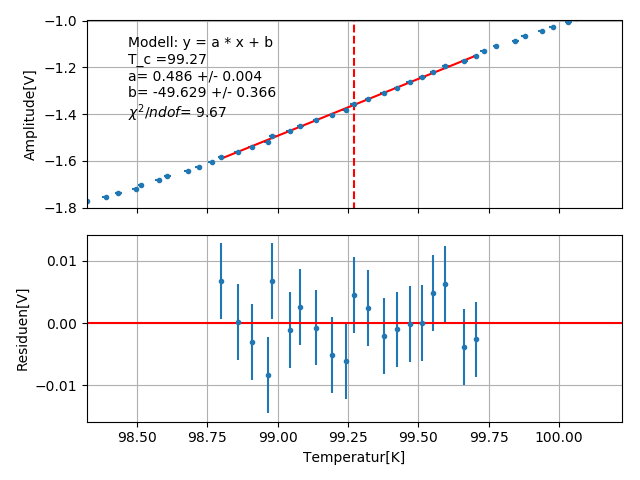
\includegraphics[scale=0.5]{Bilder/Haupt_Supra/X1_Steigung2.png}
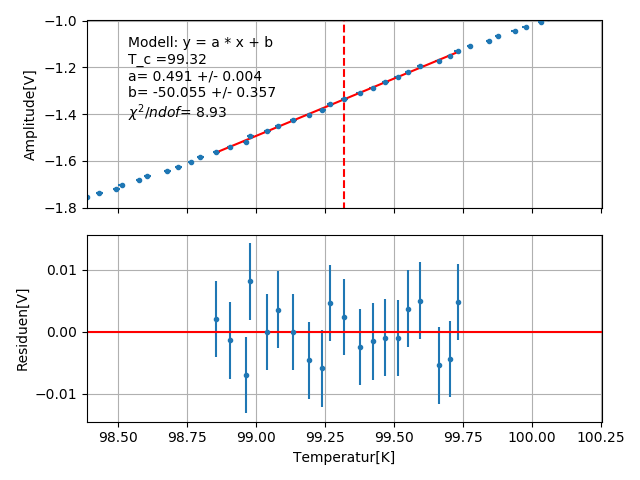
\includegraphics[scale=0.5]{Bilder/Haupt_Supra/X1_Steigung3.png}
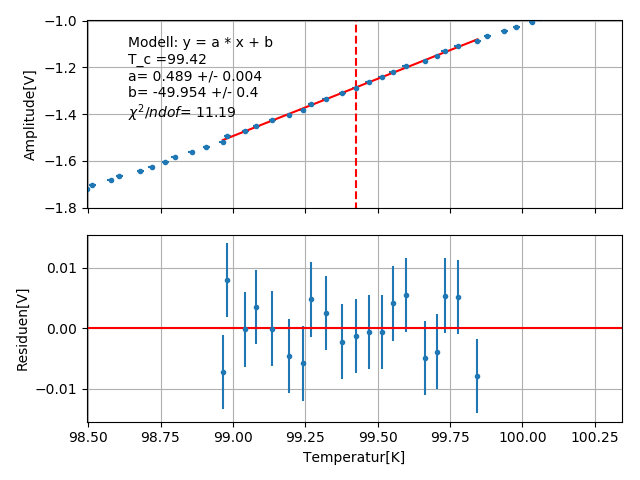
\includegraphics[scale=0.5]{Bilder/Haupt_Supra/X1_Steigung4.png}
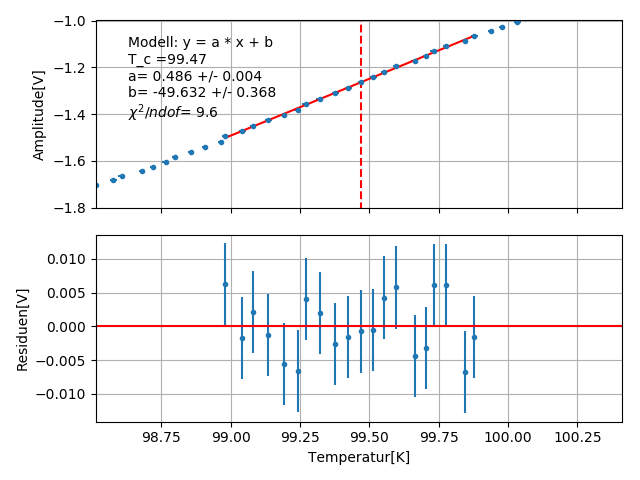
\includegraphics[scale=0.5]{Bilder/Haupt_Supra/X1_Steigung5.png}

\caption{Anpassungen an den Datenpunkt, die die größte Steigung ergeben hat (oben) und Anpassungen an die benachbarten Datenpunkte. Die zur Anpassung gehörigen Temperaturen $T_C$ wueden mit einer senkrechten Linie markiert.}
\label{fig:Supra_X1anpass}
\end{figure}

\begin{figure}
\centering
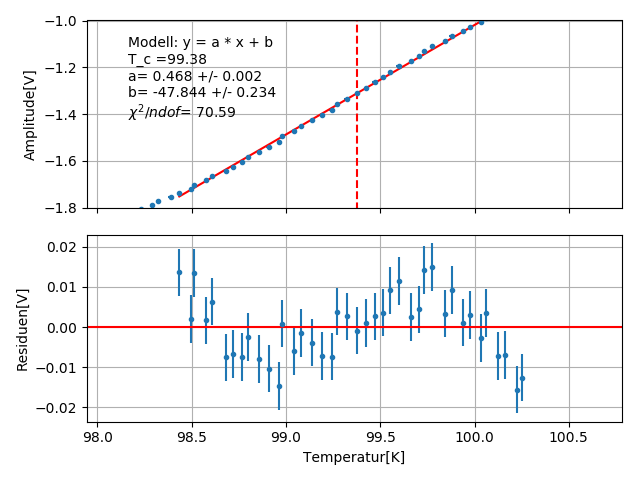
\includegraphics[scale=0.8]{Bilder/Haupt_Supra/X1_Steigung20.png}
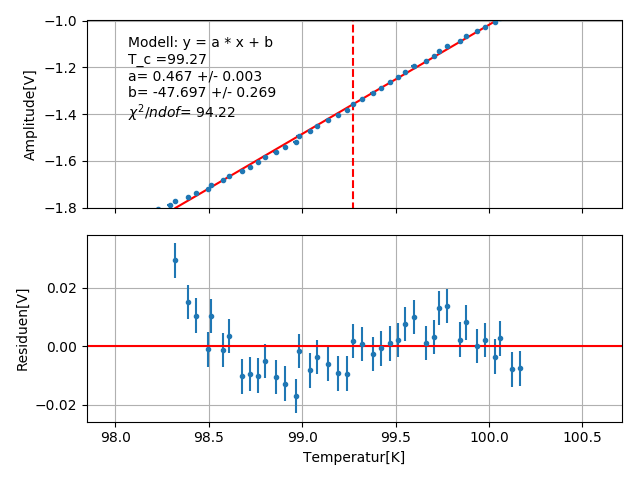
\includegraphics[scale=0.5]{Bilder/Haupt_Supra/X1_Steigung21.png}
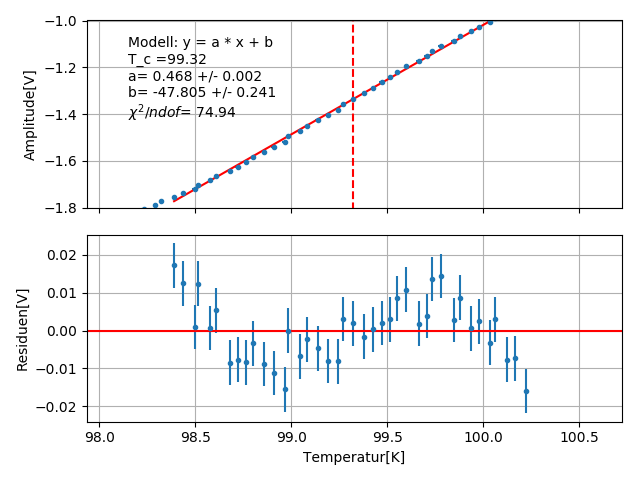
\includegraphics[scale=0.5]{Bilder/Haupt_Supra/X1_Steigung22.png}

\caption{Visualisierung der Folgen eines größeren Anpassungsbereiches (20 Nachbarpunkte) (oben: Maximalstelle, unten: nächste Nachbarn der Maximalstelle). Es ergibt sich die selbe Maximalstelle, allerdings ist in den Residuen eine Systematik zu erkennen, weswegen ein größerer Anpassungsbereich keinen wirklichen Sinn macht.}
\label{fig:Supra_X1anpassgross}
\end{figure}

\paragraph{Temperaturgradient}
\begin{figure}
\centering
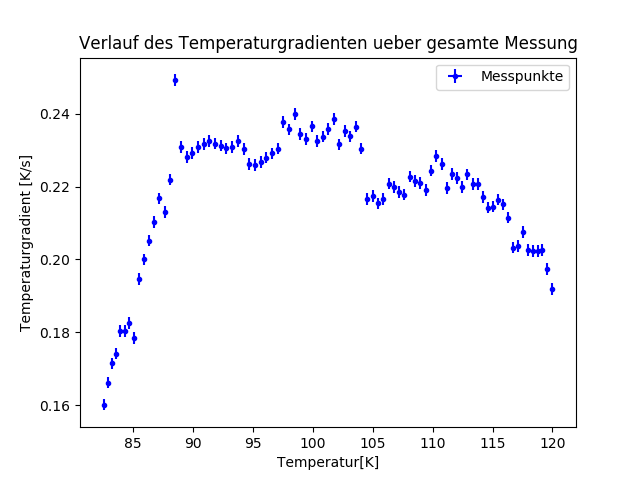
\includegraphics[scale=0.8]{Bilder/Haupt_Supra/X1_temp.png}
\caption{Temperaturgradient der $\chi'$-Messung.}
\label{fig:Supra_X1_temp}
\end{figure}

In Abbildung \ref{fig:Supra_X1_temp} ist der Temperaturgradient der Messung in Abhängigkeit von der Temperatur dargestellt. Im relevanten Bereich zwischen 98-100K erhält man durch eine Mittelung (Fehler aus Fehler auf den Mittelwert) eine ungefähre Abschätzung des Temperaturgradienten, der für die Abschätzung der Sprungtemperatur eine Rolle spielt:
\begin{equation*}
\dfrac{dT}{dt} = \SI{0.236\pm 0.005}{K/s}
\end{equation*}

\newpage
\subsubsection{Auswertung der $\chi''$-Messung}
\begin{figure}[h]
\centering
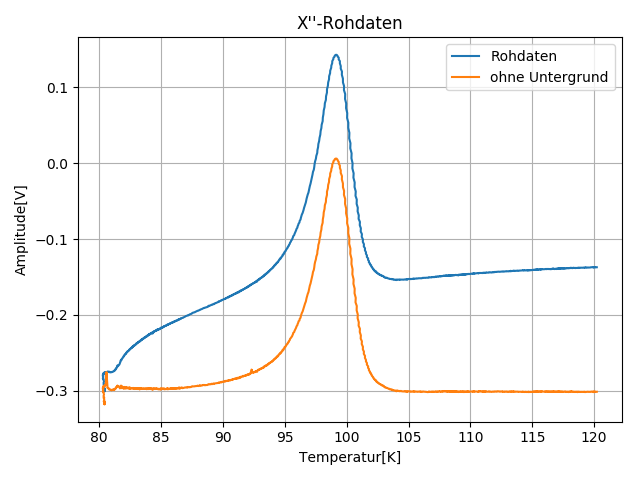
\includegraphics[scale=0.8]{Bilder/Haupt_Supra/X2roh.png}
\caption{Rohdaten und vom Untergrund bereinigte Daten der $\chi''$-Messung.}
\label{fig:Supra_X2roh}
\end{figure}

Die $\chi''$-Messung wurde ebenfalls vom Untergrund bereinigt. Dies ist zusammen mit den Rohdaten in Abbildung \ref{fig:Supra_X2roh} dargestellt.\\
\\
\paragraph{Kuvenverlauf}
Der Verlauf der $\chi''$-Messung kann folgendermaßen erklärt werden:\\
Da der Supraleiter leitend ist wird ein Strom in der Probe induziert. Durch die Änderung der Suszeptibilität ändert sich auch die Induktivität und somit die Spannung, die wieder in der Spule induziert wird. Diese Spannung ist um $90^\circ$ phasenverschoben und kann deswegen im Imaginärteil betrachtet werden. Je stärker die Änderung der Suszeptiblität ist, desto größer ist diese Spannung. Es entsteht ein Peak um die Sprungstelle.
\paragraph{Sprungtemperatur}
Die Sprungtemperatur stimmt hier mit der Peakposition überein. Um diese Postition zu bestimmen wird eine quadratische Funktion an die Spitze des Peaks angepasst. Der Fehler bestimmt sich durch Variation des Anpassungsbereiches, da durch die Unterschiedliche Flankensteigung des Peaks eine Systematik das Ergebnis ungenauer macht und deswegen der Fehler aus den Anpassungen auf die Position unter Umständen zu klein ist.\\
In Abbildung \ref{fig:Supra_X2anpassung} sind Anpassungen mit 3 verschiedenen Bereichen um die Peakspitze herum gezeigt. Die Ergebnisse dieser Anpassungen werden gemittelt. Den Fehler erhält man durch die maximale Abweichung einer Anpassung vom Mittelwert. Daraus ergibt sich das Endergebnis von
\begin{equation*}
T_C = \SI{99.12\pm 0.02}{K}
\end{equation*}

\paragraph{Temperaturgradient}
Mit der gleichen Methode wie bei der $\chi'$-Messung kann man hier den Temperaturgradienten bestimmen. Dies ist in Abbildung \ref{fig:Supra_X2temp} dargestellt. Es ergibt sich durch Mittelung der Werte zwischen 98K und 100K wieder ein relevanter Wert von 
\begin{equation*}
\dfrac{dT}{dt} = \SI{0.213\pm 0.004}{K/s}
\end{equation*}

\begin{figure}
\centering
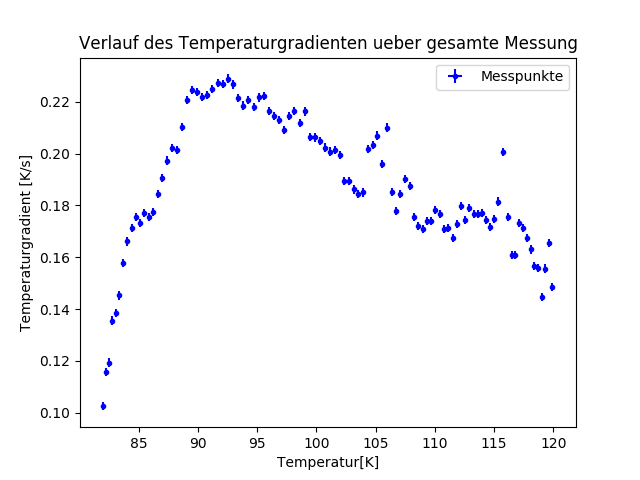
\includegraphics[scale=0.8]{Bilder/Haupt_Supra/X2_temp.png}
\caption{Temperaturgradient der $\chi''$-Messung.}
\label{fig:Supra_X2temp}
\end{figure}

\begin{figure}
\centering
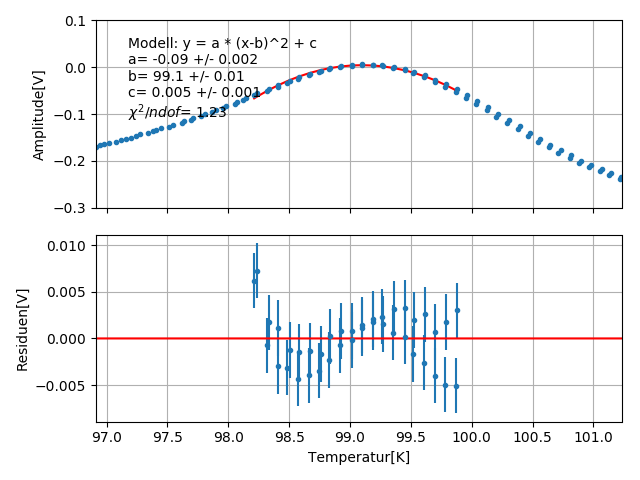
\includegraphics[scale=0.6]{Bilder/Haupt_Supra/X2_anpassung1.png}
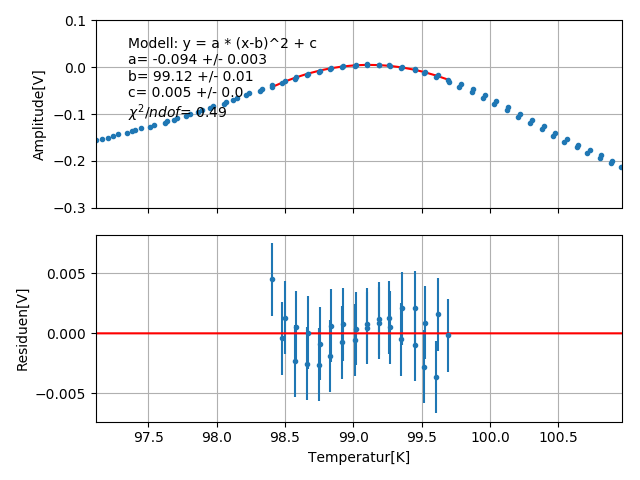
\includegraphics[scale=0.6]{Bilder/Haupt_Supra/X2_anpassung2.png}
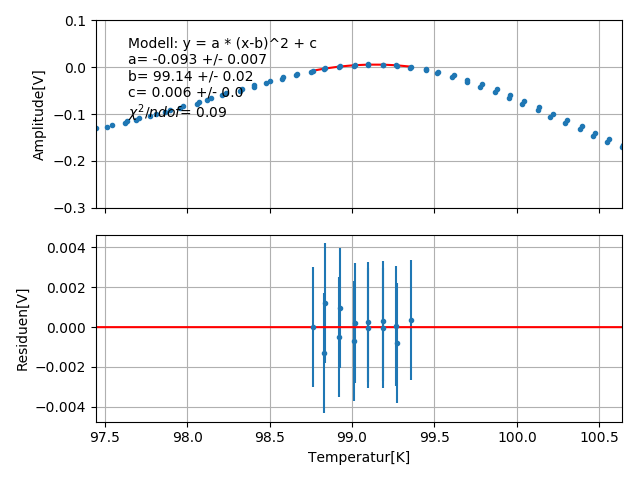
\includegraphics[scale=0.6]{Bilder/Haupt_Supra/X2_anpassung3.png}

\caption{Anpassungen an die Peakspitze mit 3 unterschiedlichen Anpassungsbereichen (14 Punkte, 28 Punkte und 40 Punkte).}
\label{fig:Supra_X2anpassung}
\end{figure}

\newpage
\subsubsection{Zusammenfassung der Messergebnisse}
Mithilfe der in der Versuchsanleitung gegebenen Daten für die Parameter des Aufbautes kann man den erwarteten Verstärkungsfaktor berechnen:
\begin{equation}
C = \dfrac{2\pi f_R \mu_0 I_0 N_{sek} N_{prim}}{l_{sek} l_{prim}}
\end{equation}
mit $f_R = \SI{380}{Hz}$,$I_0 = \SI{1}{mA}$,$N_{sek} = 700$,$N_{prim} = 2046$,$l_{sek} = \SI{20}{mm}$,$l_{prim} = \SI{50}{mm}$. Das Ergebnis ist in Tabelle \ref{tab:supra_ergebnis} zu finden.\\
Das Messergebnis weicht sehr stark vom Erwartungswert ab. Dies kann mehrere Gründe haben:
\begin{enumerate}
\item Fehler in der Methode zur Messwertbestimmung:\\
Es kann zum Beispiel sein, dass die Plateaus nicht den zugeordneten Suszeptiblitäten entspechen, sondern z.B die Suszebtiblität im supraleitenden Zustand $<1$ ist.
Dies ist zwar grundsätzlich möglich, es gibt aber eine Beobachtung, welche die Größenordnung des Messergebnisses bestätigt und eher den Erwartungswert hinterfragt:\\
Mithilfe von 
\begin{equation}
U_{max}^{lit} = C_{lit} \cdot \chi_{max} \cdot v \cdot (1-n_m) \cdot V_{Probe}
\end{equation}
und den verwendeten Werten für die SChnellauswertung während des Versuches von $\chi_{max} = 5$, $v = 20000$, $n_m = 0.27$ und $V_{Probe} = 22.9mm^3$ ergibt sich eine maximale Spannung von $U_{max} = 7.18V$. Mit dem sich aus der Messung ergebenen Wert für die Kalibrationskonstante ergibt sich hingegen eine Spannung von $U_{max} = 13.48V$. Bei der Messung mit diesen Einstellungen wurden Spannungen von über 10V erreicht, weswegen der Verstärkungsfaktor angepasst werden musste. Dies spricht eher für den berechneten Wert und gegen den Literaturwert.
\item Veraltete oder falsche Daten zur Berechnung des Erwartungswertes:\\
Da die Versuchanleitung schon etwas älter ist, kann auch nicht ausgeschlossen werden, dass die angegebenen Werte für veraltete Bauteile oder Proben gelten, wodurch sich ein anderer Kalibrationsfaktor ergibt. Dies ist wegen der oben ganannten Beobachtung wesentlich wahrscheinlicher.
\end{enumerate}

\begin{table}
\centering
\begin{tabular}{|c|c|c|}
\hline 
Messwert & Messergebnis & Erwartungswert \\
\hline 
Kalibrationskonstante C & $8034.2\pm 34.7$ & $4297$ \\ 
\hline 
Sprungtemperatur $\chi'$ & \SI{99.12\pm 0.02}{K} & \SI{92}{K} \\ 
\hline 
Sprungtemperatur $\chi''$ & $(99.38^{+0.04}_{-0.06}) K$ & \SI{92}{K} \\ 
\hline 
\end{tabular} 
\caption{Zusammenfassung der Messergebnisse zum Supraleiter und die dazu gehörigen Erwartungswerte.}
\label{tab:supra_ergebnis}
\end{table}

\paragraph{Sprungtemperatur}
Der Literaturwert der Sprungtemperatur des verwendeten YBaCuO-Supratleiters beträgt 92K \footnote{https://de.wikipedia.org/wiki/Yttrium-Barium-Kupferoxid}. Die beiden Messwerte zur Sprungtemperatur weichen also um c.a 7K von der Erwartung ab. Dies ist vor allem dem Offset verschuldet, der dadurch entsteht, dass sich das Thermometer schneller erwärmt als die Probe. Der große Temperaturgradient führ zu diesem relativ großen Offset. Durch die leicht unterschiedlichen Temperaturgradienten bei den beiden Messungen kann ebenfalls erklärkt werden, dass das Ergebnis für die $\chi'$ Messung etwas größer ist.
\subsection{Messung der Probe}

\section{Fazit}

\end{document}
